\documentclass[10pt]{article}
\usepackage[T1]{fontenc}
\usepackage[utf8]{inputenc}
\usepackage[a4paper,margin=25mm]{geometry}
\usepackage{lmodern,microtype,amsmath,amssymb,amsthm}
\usepackage{graphicx,booktabs,array,tabularx}
\usepackage[numbers,sort&compress]{natbib}
\usepackage[colorlinks=true,allcolors=blue]{hyperref}
\newcommand{\R}{\mathbb{R}}
\newcommand{\spec}{\operatorname{spec}}
\newcommand{\rank}{\operatorname{rank}}
\newcommand{\im}{\operatorname{im}}
\newcommand{\diag}{\operatorname{diag}}
\renewcommand{\thesection}{S\arabic{section}}
\renewcommand{\theequation}{S\arabic{equation}}
\renewcommand{\thetable}{S\arabic{table}}
\renewcommand{\thefigure}{S\arabic{figure}}
\setlength{\parskip}{3pt}
% Generated by scripts/summarize_study.py; do not transcribe historical metrics here.
\newcommand{\StudyProteins}{364}
\newcommand{\StudyResidues}{78,400}
\newcommand{\StudyClusters}{349}
\newcommand{\GraphPCC}{0.625}
\newcommand{\NativePCC}{0.611}
\newcommand{\NativeGraphPCC}{0.628}
\newcommand{\CenterPCC}{0.565}
\newcommand{\CombinedPCC}{0.627}
\newcommand{\CombinedCILow}{0.613}
\newcommand{\CombinedCIHigh}{0.641}
\newcommand{\DeltaPCC}{+0.0018}
\newcommand{\DeltaCILow}{-0.0009}
\newcommand{\DeltaCIHigh}{+0.0044}
\newcommand{\AbstractEmpiricalResults}{The graph baseline attained mean per-protein correlation $0.625$, while adding corrected center-zero degree-zero spectra yielded $0.627$ (paired difference $+0.0018$; 95\% cluster-bootstrap interval $[-0.0009,+0.0044]$). The primary comparison does not resolve an improvement in mean correlation under this evaluation.}

\title{Supplementary material\\\large Interpreting Local Sheaf Spectra for Protein B-Factor Prediction}
\author{Ryan Charette\\\small Independent researcher}
\date{}
\begin{document}
\maketitle

\section{Scope and notation}
This supplement specifies the calculations supporting the operator characterization and provides the detailed policies connecting structures to benchmark rows. It accompanies the regenerated experiment; older metric snapshots and manuscript drafts are not treated as interchangeable evidence. The primary article defines the cochain convention: $d_q$ maps $q$-simplex assignments to $(q+1)$-simplex assignments, and all displayed matrices use orthonormal simplex bases. This makes matrix transpose the adjoint. Reversing a simplex orientation changes signed basis vectors and yields orthogonally equivalent operators; changing a stalk metric generally changes the numerical spectrum.

\section{The universal-center spectrum in a broader form}
Let $H$ be an arbitrary unweighted graph on $m\geq1$ vertices, and attach one center to every vertex of $H$ by an edge of common weight $t>0$. The weighted Laplacian is
\begin{equation}
L_t=\begin{pmatrix}tm&-t\mathbf1^T\\-t\mathbf1&L_H+tI\end{pmatrix}.
\end{equation}
The orthogonal decomposition
\begin{equation}
\R^{m+1}=\operatorname{span}\{(1,\mathbf1)^T\}
\oplus\operatorname{span}\{(m,-\mathbf1)^T\}
\oplus\{(0,v)^T:v\perp\mathbf1\}
\end{equation}
is invariant under $L_t$. The three restrictions have eigenvalues $0$, $t(m+1)$, and $t+\lambda_j(H)$ for $j=2,\ldots,m$, respectively. Choosing one all-ones eigenvector for $\lambda_1(H)=0$ leaves any additional neighbor-component zero modes inside the last subspace. They become eigenvalues $t$, rather than extra zero eigenvalues. Thus the universal center makes the graph connected irrespective of whether its neighbors connect to one another.

For the native setting $t=2$, $\lambda_j(H)\leq m$ implies the largest eigenvalue is $2(m+1)$. A short proof of the bound uses the complement graph: on $\mathbf1^\perp$, $L_H+L_{\overline H}=mI$, and both Laplacians are positive semidefinite. The trace is $2|E(H)|+4m$, yielding positive-spectrum mean $4+2|E(H)|/m$. With $t=1$, the corresponding maximum is $m+1$ and mean is $2+2|E(H)|/m$. These results apply to the complete spectrum, not only to asymptotic approximations. A solitary center has the separate spectrum $\{0\}$.

The other summaries cannot generally be reduced to those two counts. Let the neighbor graph be either the four-vertex path $P_4$ or the three-leaf star $K_{1,3}$, both with four vertices and three edges. Adding the native weight-two universal center gives the respective positive spectra
\begin{equation}
\{4-\sqrt2,4,4+\sqrt2,10\},\qquad \{3,3,6,10\}.
\end{equation}
Both operators have nullity one, maximum ten, and positive mean $11/2$. Their minima differ, their medians are $4+\sqrt2/2$ and $9/2$, and their positive population standard deviations are $\sqrt{31}/2$ and $\sqrt{33}/2$. Thus minimum, median, and standard deviation retain distinctions beyond neighborhood size and neighbor-edge count.

Both graphs are realizable by the local Euclidean rule, so this counterexample applies within the construction's geometric scope. With target at the origin and cutoff $R=1$, place the path neighbors at radius $0.9$ and planar angles $0,60,120,180$ degrees. Only consecutive neighbors are within the cutoff. For the star, use neighbor hub $(0.1,0,0)$ and leaves $(0,0.9,0)$, $(0,-0.45,0.45\sqrt3)$, and $(0,-0.45,-0.45\sqrt3)$. Every target distance is below one; hub--leaf distances are $\sqrt{0.82}<1$ and leaf--leaf distances are $0.9\sqrt3>1$. These are theoretical examples, separate from the protein benchmark.

The historical native attenuation parameter $p$ divides edge weights by a distance-dependent factor when $p>0$. Such reweighting is a graph operation, not persistence between complexes. The previous higher-degree interface combined a weighted vertex--edge incidence matrix with an unweighted triangle boundary. For a triangle $[c,u,v]$ with the native center weights, its degree-zero coboundary rows were
\begin{equation}
D_0=\begin{pmatrix}-\sqrt2&\sqrt2&0\\-\sqrt2&0&\sqrt2\\0&-1&1\end{pmatrix},
\qquad D_1=(1,-1,1),
\end{equation}
so $D_1D_0=(0,\sqrt2-1,1-\sqrt2)\ne0$. The revised native interface therefore rejects weighted higher-degree requests, and the native comparator is confined to degree zero. This incompatibility does not affect the positive-semidefinite graph interpretation of $D_0^TD_0$; the compatible higher-degree experiments use the separately defined alpha-complex sheaf operators.

\section{Weighted deletion and augmented link}
For the center-zero geometric sheaf, order simplices by whether they contain $c$. A restriction crossing from a simplex without $c$ to a coface with $c$ vanishes, while the reverse containment is impossible. Therefore the cochain complex splits orthogonally. Within the deletion, all labels are one and the restriction is $F(\sigma)/F(\tau)$. Define $T_q$ to multiply the coordinate on $\sigma$ by $F(\sigma)$. Then
\begin{equation}
T_{q+1}d_qT_q^{-1}=d_q^{\mathrm{ordinary}}.
\end{equation}
Since every $F(\sigma)>0$, this is an invertible cochain identification. It proves equality of cohomology dimensions, but $T_q$ need not be orthogonal. Consequently it does not replace the weighted Laplacian spectrum by an unweighted spectrum under the original inner product.

For the center-containing block, write each simplex as $c*\sigma=\{c\}\cup\sigma$, put $c$ first in the orientation, and define $G(\sigma)=F(c*\sigma)$. The induced link restriction is $G(\sigma)/G(\tau)$. The empty simplex belongs to the augmented link complex, has degree $-1$, and corresponds to $c$. In particular, $G(\emptyset)=F(c)=1$, and the map from the empty simplex to a link vertex $v$ has coefficient $1/r_{cv}$. Omitting that map would incorrectly remove the center scalar from the degree-zero sheaf operator.

A signed permutation between center-containing simplices and augmented link simplices preserves the Euclidean inner product, giving a spectral identification with this \emph{weighted} augmented link complex. Multiplication by $G$ then supplies a separate, generally nonorthogonal identification with ordinary augmented link cochains. Hence the zero multiplicities are governed by reduced link cohomology. For a nonempty link, $\widetilde H^{-1}(J)=0$; for a link with no vertices, the augmented complex retains the empty-simplex coordinate and $\widetilde H^{-1}(J)=\R$. This yields
\begin{equation}
\dim\ker L_q=\beta_q(D)+\widetilde\beta_{q-1}(J),\qquad q\geq0,
\end{equation}
with that convention at degree zero. In degree one, the link contribution counts independent component differences, not the link's ordinary un-reduced component count.

This derivation is a direct specialization of compatible weighted/sheaf complexes, in relation to prior relative sheaf theory \citep{hansen2019}, weighted homology \citep{renwu2021}, and local/link Laplacian constructions \citep{liu2026}. It is included to interpret this molecular representation and verify its implementation; it is not presented as a new general local-homology theorem.

\section{Persistent operator and independent matrix checks}
Write $D_q^b=[A\ B]$ with columns indexing old and new $q$-simplices. A vector $z$ in $(q+1)$-cochains has adjoint coboundary supported on the old simplices precisely when $B^Tz=0$. If the columns of $Z$ form an orthonormal basis of $\ker B^T$, the persistent coboundary has matrix $Z^TA$, and its upper Laplacian is $A^TZZ^TA$. Singular-value decomposition gives $ZZ^T=I-BB^\dagger$. This proves the projector form without forming normal equations.

Let $H=(D_q^b)^TD_q^b$. Because $B(B^TB)^\dagger B^T=BB^\dagger$, the projector form equals
\begin{equation}
H_{AA}-H_{AB}H_{BB}^\dagger H_{BA}.
\end{equation}
The lower term is formed from $d_{q-1}$ on the lower complex. In degree one this is $D_0^a(D_0^a)^T$, on the old edge space. Substituting the upper-complex lower term would generally change dimensions or the intended pair. The derivation follows the generalized Schur-complement principle for persistent Laplacians and its sheaf counterpart \citep{memoli2022,wei2025}.

Positive semidefiniteness follows directly from $x^TA^TZZ^TAx=\|Z^TAx\|^2$. When there are no new $q$-simplices, $B$ has zero columns and $ZZ^T=I$. When there are no old $q$-simplices, the output is the empty operator. At equal endpoints, the ordinary sheaf Laplacian is recovered. The implementation checks these limits, compares the Schur operator with a nullspace-based construction, and checks numerical symmetry and eigenvalues. The reported rank tolerance is part of the computation: forming $B^TB$ squares singular values, so its threshold must be interpreted consistently rather than copied blindly from an SVD threshold on $B$.

For the center-zero sheaf, the old/new ordering can be refined by center membership. Both $A$ and $B$ are then block diagonal with respect to the two independent cochain complexes. Orthogonal projection onto $\ker B^T$ respects the same split, and so does the persistent operator. This justifies comparing the union of block spectra with the full spectrum at nonzero width. It does not justify using an independently chosen metric for the link block.

At degree zero, every scale in the fixed-support alpha filtration has exactly the same vertex set. The new-vertex column block is empty, and $L_0^{a,b}=L_0^{b,b}$. This identity relies on the fixed support and common restrictions. It need not hold when vertices are introduced during a filtration, neighborhoods are rebuilt independently at each scale, or stalks change between complexes. It explains the present choice to use degree one for the positive-width experiment.

\section{Structure selection and identity audit}
Only the first PDB model is analyzed. Standard amino acids and modified residues recognized by Biopython's extended protein-residue mapping contribute one selected C-alpha atom. Selenomethionine is mapped to methionine in the observed sequence; SEC, PYL, and UNK are represented as X. Twelve additional components classified as D-peptide linking by the Chemical Component Dictionary \citep{ccd} are retained geometrically and represented as X, without asserting an L-amino-acid parent identity: DIV, DAL, DPN, DVA, DCY, DPR, DGL, DTR, DAR, DLE, DAS, and DLY. The three-letter identities remain available in the residue audit. The installed mapping and component-specific source links are recorded in the configuration.

Nonpolymer components CA, PLM, and MPT are explicitly excluded, even where the supplied coordinate file labels their records ATOM. An atom name of CA alone does not establish a protein C-alpha. The final audit retains 78,400 residues in 364 structures and excludes 19 nonpolymer records from the historical 78,419-row collection: 16 calcium ions, one PLM record, and two MPT records. Relative to an initial standard-residue audit, this policy restores 177 modified or D-peptide residues before fitting any model. Geometry includes these retained coordinates; unrecognized components receive no generic carbon-atom fallback.

Among alternate C-alpha locations, choose the highest occupancy, breaking ties by blank alternate-location code, then A, then lexical order. Duplicate records with the same residue and alternate-location key are treated as an error. The element field must be carbon or blank; a conflicting explicit element is rejected.

Nonfinite coordinates, occupancies, or B-factors and negative occupancies or B-factors are rejected. Structures with fewer than three retained C-alpha atoms or constant retained B-factors are excluded from correlation-based prediction. Each selected row preserves the structure, model, chain, residue number, insertion code, atom selection, and source hash. Coincident coordinates require an explicit geometry check before restrictions dividing by distance can be computed. A preprocessing exclusion and a numerical feature-generation failure are separate audit categories.

Normalized B-factor is computed over the complete retained protein entry, with population standard deviation, and is never a feature. Legacy annotation tables are excluded from the primary feature matrix because a supplied residue index alone does not establish a verified chain/residue mapping. Source annotation correlations from historical analyses therefore are not claimed as validation of the new model. The present primary target and all predictors come from the audited structure rows.

\section{Observed-sequence clustering and fold assignment}
Observed sequences are assembled separately for each chain. Biopython local pairwise alignment uses BLOSUM62, gap opening $-10$, gap extension $-0.5$, and the first optimal alignment returned by the fixed implementation. Identity is the number of exactly matching non-X residue pairs divided by the number of aligned nongap residue pairs. Coverage for each chain is the same nongap pair count divided by that chain's observed length. Thus X contributes to the denominator when aligned but does not count as an identity match. A chain pair qualifies at identity $\geq0.30$, reciprocal coverage $\geq0.80$, and at least 50 aligned nongap residue pairs.

Any qualifying chain pair links the corresponding whole protein entries. Exact complete chain-sequence multiset duplicates are also linked irrespective of size; unknown positions use their explicit three-letter residue identities for this duplicate check, preventing distinct X-coded components from becoming artificial matches. Identical small auxiliary chains alone do not activate the exception. Connected components define the final grouping. This is conservative with respect to proteins sharing a qualifying chain and allows chains within a multimer to keep their common structural context. It is not a claim that a 30\% threshold alone establishes or excludes evolutionary homology. Entries containing only chains shorter than 50 residues rely on the complete-sequence duplicate rule and receive no assurance against more distant sequence similarity.

The initial grouping rule used coverage of only the shorter chain and had no minimum aligned length. On the initial standard-residue audit, it produced 3,434 edges and a single component containing all 364 eligible entries, driven by transitive bridges through very short auxiliary fragments. Before prediction outcomes were accessed, the rule was amended to the reciprocal-coverage and minimum-length definition above. After the final chemical-identity audit, the graph has 16 edges and 349 components: 336 singletons, 11 pairs, and two triplets. The final chain audit records 565 observed chains, of which 108 are shorter than 50 residues; 47 entries have only such short chains, and 119 entries have multiple chains. Both the original graph and the amendments are retained as protocol evidence. These audited counts describe the grouping process, not a measured improvement in prediction.

Cluster components are sorted by decreasing total residue count, with a seeded SHA-256 tie-breaking key. In order, each is assigned to the currently least-loaded of five folds, breaking load ties by numeric fold identifier. Ordinary protein-only folds use the same rule on individual proteins. The assignment is deterministic and label-free. A fold manifest is shared across feature families, so a comparison cannot improve by drawing a more favorable partition. The bootstrap resamples the resulting whole clusters 2,000 times, conditional on the held-out predictions, and recomputes the macro-protein estimand in every resample.

Pearson and Spearman correlations are marked undefined if fewer than three paired residues are available or the target or prediction has standard deviation at most $10^{-12}$. Such entries remain in prediction and RMSE tables but contribute no finite correlation to its macro mean. Each metric summary records its number of valid proteins; paired correlation differences use only proteins with finite values for both models. The bootstrap first retains finite values for the specified estimand, then samples whole remaining clusters with replacement and reports the 2.5th and 97.5th percentiles of the resulting protein means. Invalid predictions or unmatched protein cohorts cause an error instead of silent row deletion.

\section{Ordered graph and spectral features}
The graph baseline has 13 columns. For each distance $r\in\{6,8,10,12\}$~\AA, it contains the nonself contact count and count divided by $n_p-1$. Two additional columns are local clustering coefficients at 8 and 12~\AA: among the center's contact neighbors, count present neighbor--neighbor edges using the same cutoff and divide by the number of possible pairs; neighborhoods with fewer than two neighbors receive zero. The final three columns are mean distances to the nearest 4, 8, and 12 nonself neighbors, using the available neighbors when a structure is shorter than the requested count. There are no B-factors, residue-position labels, inverse-square packing sums, or exponential kernels in this baseline.

The new spectral-output convention is numerical nullity, smallest positive eigenvalue, largest positive eigenvalue, positive mean, positive median, and positive population standard deviation, in that order. All six are computed at each declared scale or pair. A spectrum with no positive eigenvalues has zero for the five positive-spectrum summaries. A zero-dimensional cochain space has zero nullity as well. Finite positive eigenvalues near the numerical tolerance require audit because changing their classification affects the minimum and zero count simultaneously. The exact tolerances are reported by the implementation metadata and matrix validation artifacts.

Native degree-zero features contain 18 columns from radii 6/9/12~\AA. Each corrected degree-zero sheaf contributes 24 columns from alpha radii 3/4/5/6~\AA\ with support 13~\AA. The core combined dimensions are therefore 31 for graph plus native and 37 for graph plus each corrected sheaf. These dimensions are checked against feature names before fitting. For degree one, static lower-endpoint pairs $(3,3),(5,5)$, persistent pairs $(3,4),(5,6)$, and static upper-endpoint pairs $(4,4),(6,6)$ each supply 12 additional features. The corresponding combined models each have 49 features. Comparing persistent additions with upper as well as lower endpoint additions addresses the possibility that increasing scale alone accounts for a gain. This grid is not selected using prediction scores.

Eigenvalue classification uses a scale-relative threshold. For $m$ eigenvalues and machine precision $\epsilon$, the default is $\max(10^{-10},64\epsilon\max(1,m))\max_i|\lambda_i|$, with zero absolute offset. Values larger than this threshold are positive modes; negative values below its negative are an error rather than silently clipped modes. The Schur Gram matrix uses the same scale-relative rule for its pseudoinverse. The independent nullspace path uses a relative singular-value cutoff of $\sqrt{10^{-10}}$, reflecting the squaring of singular values in the Gram matrix. Additional dimension-dependent roundoff protection is recorded in the implementation. A zero spectrum is classified as zero without introducing an arbitrary absolute geometric scale.

\section{Degree-one cohort and computational limits}
The label-free timing pilot selected two proteins by seeded hash from each tercile of maximum 13~\AA\ support size, plus the preset principal case 1ULR. The selected identifiers were 1MF7, 1PMY, 1ULR, 2NUH, 2WUJ, 3M3P, and 3T47. The pilot evaluated the complete feature suite, including graph/native descriptors, degree-zero and degree-one operators, eigensolvers, and serialization. Its recorded wall time was 37.96 seconds. The pilot preceded restoration of modified peptide coordinates: extrapolating its slowest per-residue cost to the initial 78,223-residue audit, allowing four workers, and multiplying by two yielded a projected full-suite time of 1,773.57 seconds. This was below the declared 21,600-second degree-one feature budget by more than an order of magnitude. The decision selected the full 364-protein eligible cohort, whose final residue count is 78,400. The retained pilot values describe a planning projection; actual production runtime is reported separately.

Nested 60- and 20-protein fallback cohorts were prepared without using prediction outcomes, but were not selected by the pilot decision. Within every reported comparison, models use the same completed cohort and frozen fold assignments. Failed or uncompleted parameter combinations are not represented by zero features or zero performance. Runtime reports distinguish feature generation from fitting and explanation. Timing measurements depend on the stated implementation and hardware and do not establish an architecture-independent complexity bound.

\section{Attribution and figure integrity}
The explained forest is the actual cluster-held-out graph-plus-center-zero predictor, including all 200 trees. The interventional background comprises 100 distinct training residues sampled without replacement, using the training seed plus the held-out fold identifier. Both explained vectors and background vectors are explicitly converted to 32-bit floating-point precision for attribution, matching scikit-learn's prediction input precision; the original 64-bit source feature arrays and effective attribution arrays are retained with data-type and hash provenance, and model predictions from the two representations must agree exactly. The geometric operators and spectral source features are computed in 64-bit precision. Summing signed feature contributions over a declared group yields a local contribution in normalized-B-factor units. An external numerical check requires the maximum absolute difference between the model prediction and the expected value plus all feature contributions to be below $10^{-6}$. A grouped contribution is not the effect of deleting that group and retraining.

Protein 1ULR is the predetermined principal visualization and 1X3O the companion. Source-residue keys determine the mapping to coordinates. A plot should state whether its colors represent observed target, model prediction, signed feature-group contribution, or absolute attribution magnitude. An unsigned map must not be labeled a signed contribution. Secondary-structure names or functional assignments are used only when independently annotated or sourced; color and visual shape alone do not establish a hinge mechanism. Image rendering is deterministic from the deposited structure and the tabulated prediction/attribution values.

\begin{figure}[tbp]
\centering
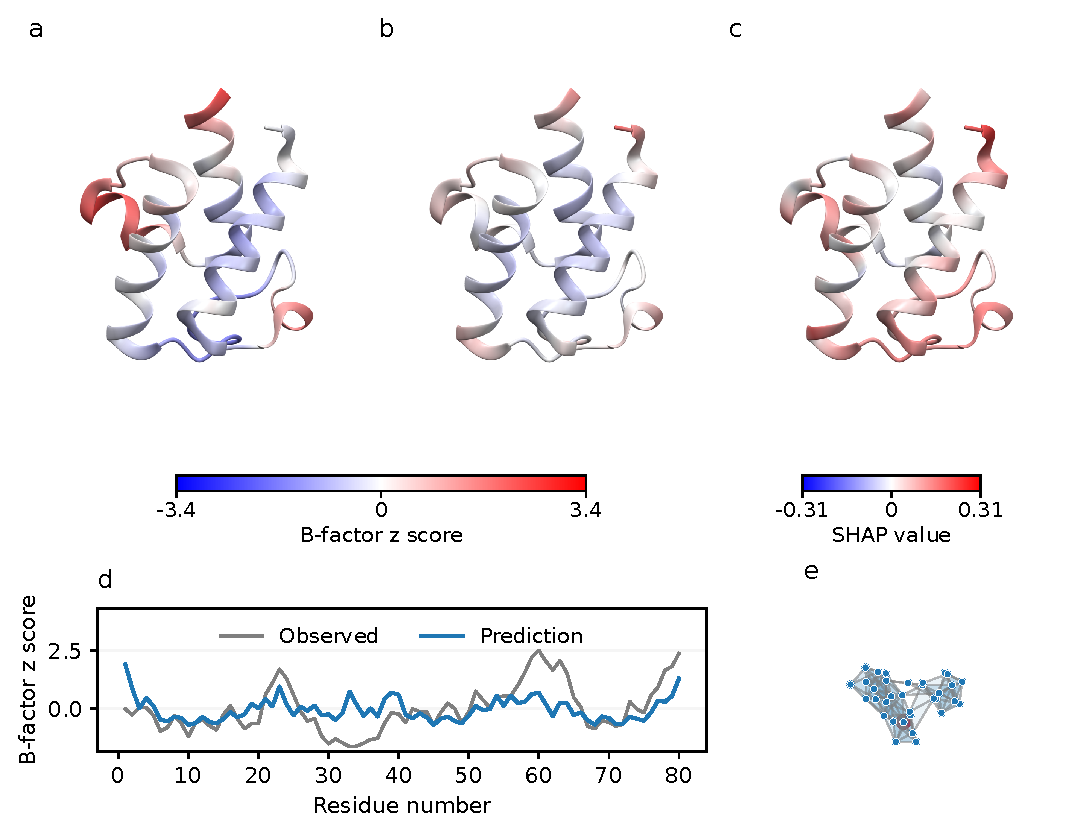
\includegraphics[width=\linewidth]{figures/supp_1X3O.pdf}
\caption{The predetermined companion protein 1X3O. (a,b) Observed within-protein normalized B-factor and the sequence-cluster-held-out graph-plus-center-zero prediction, mapped to the same residue coordinates and shown with a common color scale. (c) The signed sum of TreeSHAP contributions from the 24 center-zero spectral features, in B-factor z-score units. This subtotal excludes graph-feature contributions and the training-background expectation; teal is negative and orange positive. (d) Observed and predicted residue profiles provide a direct check alongside the structural views. (e) The local alpha complex at ball radius 4~\AA\ within the fixed 13~\AA\ support of the labeled residue. The protein, model protocol, and feature grouping were specified before inspecting prediction outcomes.}
\label{fig:companion}
\end{figure}

% Generated by scripts/summarize_study.py; do not transcribe historical metrics here.



\begin{table}[htbp]\centering\small
\caption{Degree-zero ablations of graph plus center-zero features. All models keep all graph features. The paired change is relative to the full multiscale spectral representation.}
\begin{tabular}{lrr}\toprule
Spectral summaries retained & Mean PCC [95\% CI] & Paired change [95\% CI]\\\midrule
Nullities only & 0.627 [0.613, 0.640] & -0.0005 [-0.0029, +0.0018] \\
Positive spectra only & 0.627 [0.613, 0.641] & -0.0000 [-0.0014, +0.0013] \\
Radius 3\,\AA & 0.628 [0.614, 0.641] & +0.0006 [-0.0015, +0.0026] \\
Radius 4\,\AA & 0.625 [0.611, 0.639] & -0.0025 [-0.0045, -0.0006] \\
Radius 5\,\AA & 0.628 [0.614, 0.641] & +0.0006 [-0.0016, +0.0028] \\
Radius 6\,\AA & 0.626 [0.612, 0.640] & -0.0011 [-0.0029, +0.0005] \\
\bottomrule\end{tabular}\end{table}




\begin{table}[htbp]\centering\small
\caption{Persistent-minus-static degree-one comparisons. All additions use twelve features on the same graph-plus-degree-zero baseline. Intervals are paired cluster-bootstrap intervals for mean protein PCC.}
\begin{tabular}{llr}\toprule
Sheaf & Static comparator & Paired PCC change [95\% CI]\\\midrule
Identity & Lower & -0.0004 [-0.0016, +0.0009] \\
Identity & Upper & +0.0000 [-0.0013, +0.0012] \\
Geometric & Lower & +0.0001 [-0.0011, +0.0012] \\
Geometric & Upper & +0.0011 [-0.0005, +0.0029] \\
Center-zero & Lower & +0.0004 [-0.0013, +0.0021] \\
Center-zero & Upper & -0.0005 [-0.0024, +0.0012] \\
\bottomrule\end{tabular}\end{table}




\begin{table}[htbp]\centering\small
\caption{Nonzero degree-one kernel frequencies across all 78,400 residue-centered neighborhoods. Neighborhoods are weighted equally. Identity and geometric nullities agree exactly at all evaluated scales. Equal endpoints describe the corresponding sheaf cohomology; unequal endpoints describe its persistent cohomology restriction rank.}
\begin{tabular}{lrrrr}\toprule
Radius pair (\AA) & \shortstack{Identity\\nonzero (\%)} & \shortstack{Center-zero\\nonzero (\%)} & \shortstack{Mean identity\\nullity} & \shortstack{Mean center\\nullity}\\\midrule
$(3,3)$ & 93.383 & 94.871 & 5.168 & 5.392 \\
$(4,4)$ & 83.679 & 86.844 & 3.102 & 3.488 \\
$(5,5)$ & 34.569 & 43.594 & 0.558 & 0.769 \\
$(6,6)$ & 3.221 & 6.657 & 0.039 & 0.080 \\
$(3,4)$ & 28.578 & 36.213 & 0.360 & 0.481 \\
$(5,6)$ & 0.361 & 2.140 & 0.004 & 0.022 \\
\bottomrule\end{tabular}\end{table}




\begin{table}[htbp]\centering\small
\caption{Protein-only split sensitivity analysis on the same 364 structures.}
\begin{tabular}{lrrr}\toprule
Representation & PCC [95\% CI] & Spearman & RMSE$_z$\\\midrule
Graph geometry & 0.622 [0.608, 0.636] & 0.602 & 0.789 \\
Legacy graph spectra & 0.609 [0.594, 0.623] & 0.598 & 0.848 \\
Graph + legacy spectra & 0.626 [0.612, 0.639] & 0.607 & 0.786 \\
Center-zero spectra & 0.560 [0.543, 0.576] & 0.554 & 0.877 \\
Graph + identity sheaf & 0.625 [0.611, 0.639] & 0.608 & 0.785 \\
Graph + geometric sheaf & 0.626 [0.612, 0.639] & 0.610 & 0.785 \\
Graph + center-zero sheaf & 0.624 [0.610, 0.638] & 0.608 & 0.786 \\
\bottomrule\end{tabular}\end{table}





\section{Evidence provenance}
Every empirical number in the main results should trace to a current output table and its configuration. Cohort counts trace to the inclusion and fold manifests; prediction statistics trace to per-protein held-out metrics; uncertainty traces to the declared bootstrap; case-study claims trace to residue-keyed prediction and attribution rows. The manuscript uses generated numerical inputs for this reason. Citations to earlier PSL studies describe their published results and corrections, while mathematical statements are tied to the operators defined here. Neither an older manuscript's number nor an unverified biological narrative is evidence for a new result.

\bibliographystyle{unsrtnat}
\bibliography{references}
\end{document}
